\documentclass[conference]{IEEEtran}
\IEEEoverridecommandlockouts
% The preceding line is only needed to identify funding in the first footnote. If that is unneeded, please comment it out.
\usepackage{cite}
\usepackage{amsmath,amssymb,amsfonts}
\usepackage{algorithmic}
\usepackage{graphicx}
\usepackage{textcomp}
\usepackage{xcolor}
\usepackage{url}
\usepackage{verbatim}
\usepackage{hyperref}
\usepackage[T1]{fontenc}
\def\BibTeX{{\rm B\kern-.05em{\sc i\kern-.025em b}\kern-.08em
    T\kern-.1667em\lower.7ex\hbox{E}\kern-.125emX}}
\begin{document}

\title{Developing a DVB-I Parser Library in Dart and GUI App in Flutter\\}

\author{\IEEEauthorblockN{1\textsuperscript{st} Luis Hebendanz}
\IEEEauthorblockA{\textit{M. Sc. Computer Science}\\
\textit{TU Berlin}\\
Berlin, Germany \\}
\and
\IEEEauthorblockN{2\textsuperscript{nd} Nicklas}
\IEEEauthorblockA{\textit{M. Sc. Information Systems Management} \\
\textit{TU Berlin}\\
Berlin, Germany \\}
\and
\IEEEauthorblockN{3\textsuperscript{rd} Balint Rüb}
\IEEEauthorblockA{\textit{M. Sc. Information Systems Management} \\
	\textit{TU Berlin}\\
	Berlin, Germany \\}
\and

}

\maketitle

\begin{abstract}
 In this project, we aimed to develop an efficient DVB-I parser library in Dart and a GUI app in Flutter to present TV services on Android devices.

We used the Dart programming language to write the DVB-I parser library and Google's cross-platform Flutter framework to develop the GUI app.

 However, we faced challenges in developing the GUI app in Flutter due to multiple bugs in the libraries we used and sparse documentation. Despite these challenges, we were able to develop a working app to present TV services on Android devices.

Our project demonstrates the feasibility of using Dart to write an efficient DVB-I parser library and Flutter to develop a GUI app that presents TV services on Android devices. However the challenges we faced in developing the GUI app highlight the importance of mature libraries and documentation to support developers in using these technologies. The lack of maturity in the Flutter ecosystem has compelled us to not recommend it for further projects.
\end{abstract}

\begin{IEEEkeywords}
IP-TV, DVB-I, Flutter, Dart, Cross Platform
\end{IEEEkeywords}

\section{Introduction}
In this project, we aimed to develop an efficient DVB-I parser library in Dart and a GUI app in Flutter to present TV services on Android devices. The DVB-I standard is a standards-based solution for delivering television via the internet and offers a discovery mechanism to signal and discover television services, using a set of REST APIs allowing clients to retrieve a list of services in an XML-based format. Our primary objective was to create a parser library that can efficiently handle the DVB-I service list registry and provide all the necessary information required to present the TV service in the client app. Additionally, we aimed to create an Android GUI app using Flutter that uses the DVB-I parser library to present the TV services to the user. 

The development of the DVB-I parser library involved reading the DVB-I standard and manually emulating REST requests as specified by the specification. We also familiarized ourselves with the Dart programming language and experimented with simple coding examples to gain proficiency with the language. Once we had a good understanding of the standard and the language, we designed and developed the DVB-I parser library using Dart, implementing the required REST APIs and XML parsing. 

The development of the Android GUI app using Flutter involved building an intuitive user interface to present the TV services to the user, as well as incorporating the DVB-I parser library to retrieve and display the information for each service. We faced challenges while developing the app, including multiple bugs in libraries used and sparse documentation, which affected the app's functionality and usability.

In this report, we will assess the success of our project in achieving its goals and evaluate the performance and usability of the DVB-I parser library and Android GUI app developed. We will also discuss the challenges encountered during development and recommend future improvements to enhance the overall functionality and usability of the app.

\section{Scientific Background}

This section will provide an overview of the utilized technologies and their respective functionalities.

\subsection{DVB-I Standard}

The DVB-I (DVB-Internet) standard is a specification developed by the Digital Video Broadcasting (DVB) organization for delivering linear television services over the internet.The standard defines the mechanisms to be used to find sets of linear television services delivered through broadband or broadcast mechanisms as well as methods to retrieve electronic programme data for those services.[ref to document]

The core of the specification is the Service List Registry (SLR) which provides a set of REST APIs allowing clients (TVs, Mobile, Browser) to retrieve a list of services (ServiceList) in an XML-based format including all information required to present the TV service in the client. The DVB-I standard, published by ETSI, expands upon the existing DVB Broadcast-based delivery methods, such as Terrestrial, Satellite, and Cable, to provide simpler and more accessible options for viewing both Linear and VOD Streaming services on any internet-connected device. With this open standard, users can enjoy a seamless viewing experience across multiple devices without any limitations.





\subsection{Flutter Framework}\label{AA}

What is Flutter. How does it work? Why we chose it?

Flutter is an open-source mobile app development framework developed by Google that allows developers to create high-performance, cross-platform mobile applications for iOS, Android, and other platforms from a single codebase.

Flutter uses a programming language called Dart, which is also developed by Google, and provides a rich set of pre-built UI widgets and tools that allow developers to create visually appealing and interactive mobile applications. The framework uses a reactive programming model, which means that changes in the app's state are automatically reflected in the UI, making it easy to build dynamic user interfaces.

One of the key benefits of Flutter is its hot-reload feature, which allows developers to quickly see the changes they make to the code in real-time on the app, without having to rebuild the entire application. This significantly speeds up the development process and makes it easier for developers to experiment with different UI designs and functionality.

Flutter is also known for its fast development speed and ease of use, making it an ideal choice for startups and businesses that need to quickly develop and deploy high-quality mobile applications.

In addition to mobile app development, Flutter can also be used for building desktop and web applications, thanks to its platform-independent nature. Overall, Flutter is a powerful and flexible mobile app development framework that is rapidly gaining popularity in the developer community.

\section{Architecture Overview}
\section{Flutter Architecture Overview}

Flutter is a cross-platform framework for building mobile and desktop applications. Its architecture consists of four main layers: the Dart app layer, the framework layer, the engine layer, and the platform layer. Shown in figure \ref{fig:flutter_tech_stack}.

\begin{figure}[ht]
	\centerline{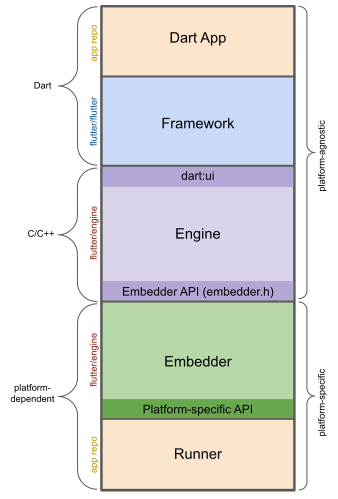
\includegraphics[width=\linewidth]{figures/app-anatomy}}
	\caption{Flutter architectural overview \cite{b1.1}}
	\label{fig:flutter_tech_stack}
\end{figure}

The Dart app layer is responsible for composing widgets into the desired UI and implementing business logic. It is owned by the app developer.

The framework layer provides a higher-level API for building UI apps, including widgets, hit-testing, gesture detection, accessibility, and text input. It composites the apps widget tree into a scene.

The engine layer is responsible for rasterizing composited scenes and provides low-level implementation of Flutter's core APIs, including graphics, text layout, and the Dart runtime. It exposes its functionality to the framework using the dart:ui API and integrates with a specific platform using the platform layer.

The platform layer ``is the native OS application that hosts all Flutter content and acts as the glue between the host operating system and Flutter``\cite{b1.1}. Flutter includes platform embedders for each of the target platforms, and you can also create a custom platform embedder.

In summary, Flutter's architecture provides a robust and efficient rendering pipeline, bypassing system UI widget libraries and using its own widget set and Skia 2D library \cite{b1.2} for rendering. This results in a high-performance, cross-platform framework with minimal abstractions and overhead.

\section{Integrating Flutter with other code}

Flutter and Dart provide several ways to integrate with other code written in different programming languages.

For mobile and desktop apps, Flutter provides platform channels, which are a mechanism for communicating between Dart code and the platform-specific code of the host app. This allows developers to call custom code written in languages like Kotlin, Swift, or C-based APIs, including those generated for code written in modern languages like Rust or Go. The platform channel mechanism serializes Dart types into a common message format, which is sent to the receiving code that then deserializes it into a programming language-specific object displayed in figure \ref{fig:platform-channels}. 

For C-based APIs, Dart provides a direct mechanism for binding to native code using the dart:ffi library, which can be considerably faster than platform channels since no serialization is required to pass data.

For web apps, the js package serves a similar purpose to dart:ffi for C-based APIs, allowing developers to bind to native code directly from Dart. Additionally, since web apps run in the browser, developers can also use Dart's interop capabilities to integrate with JavaScript libraries, either by importing JavaScript libraries into Dart or by calling Dart code from JavaScript.

\begin{figure}[ht]
	\centerline{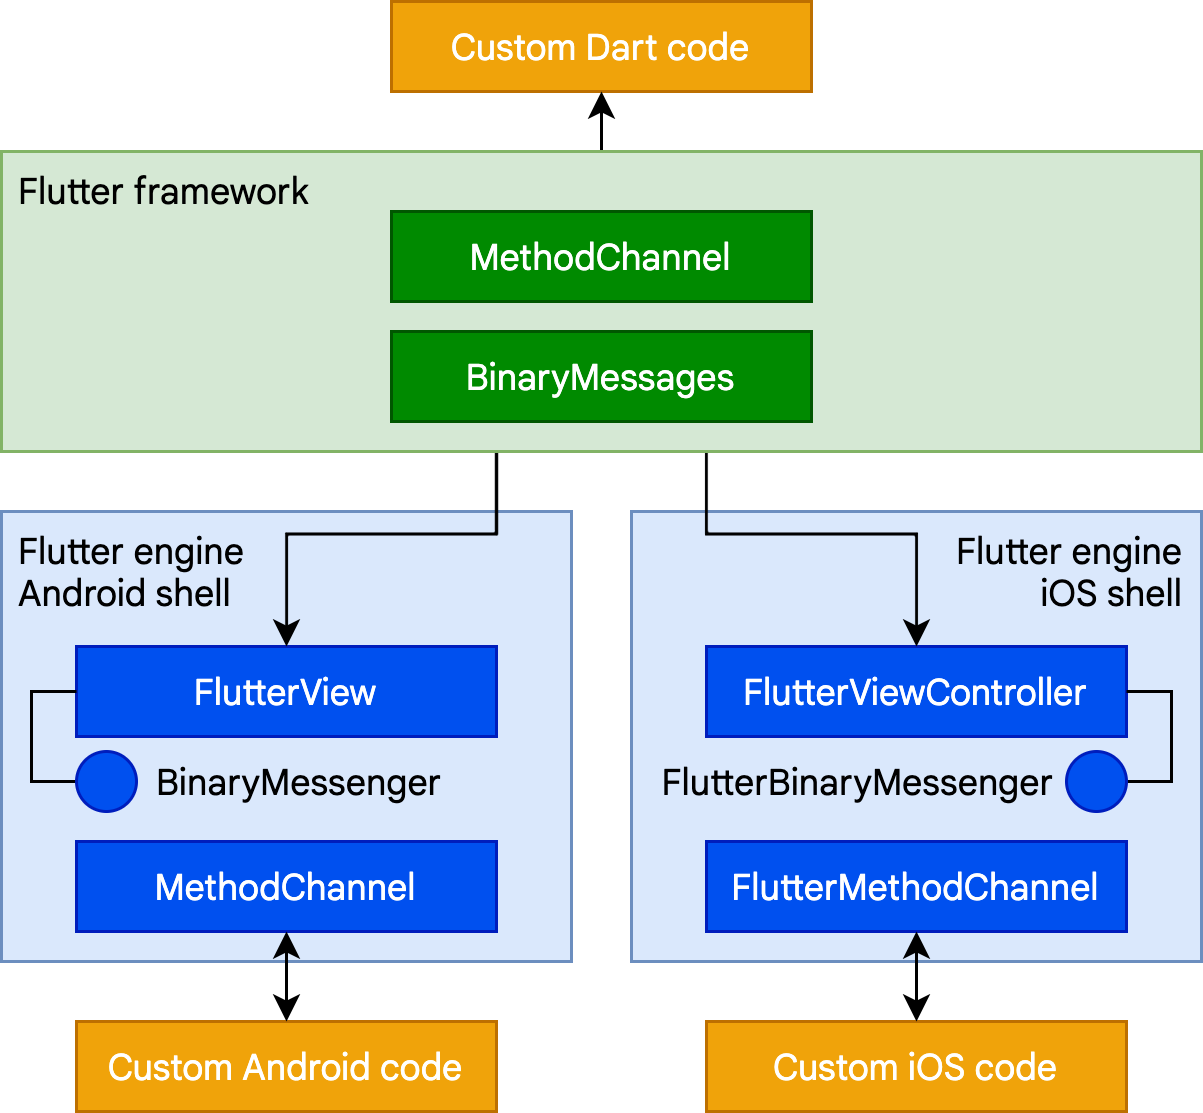
\includegraphics[width=\linewidth]{figures/platform-channels}}
	\caption{Platform Channels Overview \cite{b1.1}}
	\label{fig:platform-channels}
\end{figure}

Overall, Flutter and Dart provide a variety of interoperability mechanisms that allow developers to integrate their code with other programming languages and platforms, providing flexibility and extensibility to their applications.


\section{State Management in Flutter}
State management is an essential aspect of building robust and performant user interfaces in Flutter. The setState() method is the most straightforward way to manage state within a single widget. When called, setState() rebuilds the widget tree, which results in the updated state being reflected in the UI.

Sharing state between widgets is a common use case in Flutter applications, and it can be achieved using the setState() method by lifting the state up to a common ancestor widget seen in figure \ref{fig:state_tree}. This involves passing callbacks down the widget tree, which can be called to update the state of the ancestor widget. However, this approach can become unwieldy and result in a cluttered codebase when dealing with large and complex widget trees.


\begin{figure}[ht]
	\centerline{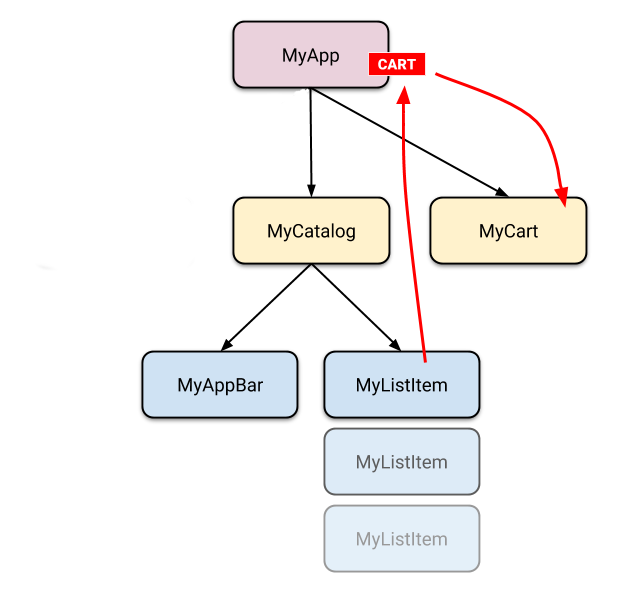
\includegraphics[width=\linewidth]{figures/state_management_tree}}
	\caption{State Tree}
	\label{fig:state_tree}
\end{figure}


The provider package offers a more robust and flexible approach to state management in Flutter applications. It provides a mechanism for sharing state across the widget tree using ChangeNotifier and ChangeNotifierProvider. ChangeNotifier is a simple class included in the Flutter SDK that provides change notification to its listeners. ChangeNotifierProvider is the widget that provides an instance of a ChangeNotifier to its descendants.

To use provider, a developer simply wraps the widget subtree that requires access to the shared state with a ChangeNotifierProvider widget. Consumers of the state can then use the Consumer widget, which listens for changes to the state and rebuilds the corresponding part of the widget tree when necessary. By using provider, developers can avoid passing callbacks down the widget tree and instead focus on building composable and maintainable widgets.



\section{Dart Language}

Dart is a class-based, object-oriented programming language with syntax that is similar to Java-style languages. It is optimized for client-side web and mobile app development, but can also be used for server-side programming. Some key concepts are:

\begin{enumerate}
	\item Everything in Dart is an object, and every object is an instance of a class.
	\item Dart has a garbage collector that automatically frees memory that is no longer in use. 
	\item Type annotations are optional in Dart because the language can infer types.
	\item If you enable null safety in Dart, variables cannot contain null values unless you explicitly make them nullable with a question mark (?).
	\item Dart does not have keywords for public, protected, and private access, however an identifier starting with an underscore (\_) is private to its library.
	\item Dart supports concurrent programming with async-await, Future, and Stream objects.
	\item A Future in Dart represents the result of an asynchronous operation and can be completed with a value or an error.
\end{enumerate}

\section{Dart Asynchronous Programming}
In Dart, async/await is a powerful mechanism that allows for writing asynchronous code in a synchronous style. With async/await, developers can write code that doesn't block the application's main event loop while waiting for I/O operations, network requests, or other time-consuming tasks to complete.

To use async/await in Dart, developers mark functions as "async" and use the "await" keyword to wait for the result of an asynchronous operation. When a function is marked as "async", it returns a Future object that can be used to obtain the result of the computation when it completes. The "await" keyword is used to wait for the Future to complete, and once it does, the result is returned as if it were a normal synchronous operation.

Async/await is particularly useful in situations where multiple asynchronous operations need to be performed in sequence, and the result of each operation is dependent on the completion of the previous one. 


\section{DVB-I Standard}

\begin{figure}[ht]
	\centerline{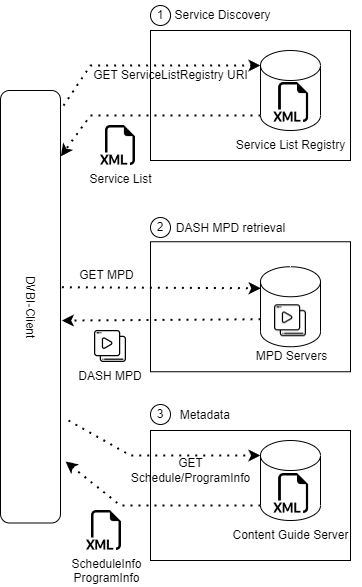
\includegraphics[width=\linewidth]{figures/DVBI-architecture.png}}
	\caption{DVBI-I architecture and client interaction overview}
	\label{dvbi-architecture}
\end{figure}

The DVB-I (Digital Video Broadcasting - Internet) \cite{DVBI-I} protocol is a standard developed by the Digital Video Broadcasting (DVB) \cite{DVB} organization. The DVB-I standard lays out processes to allow internet connected devices, such as smartphones, tablets, laptops, and smart TVs, to receive broadcast quality content, including live and on-demand TV channels. It aims to provide simpler and more accessible options for viewing both linear and Video-On-Demand (VOD) streaming services on any internet-connected device.

The DVB-I standard consists of many components. Figure \ref{dvbi-architecture} illustrates the elements most relevant to our project. At the core of the DVB-I protocol is the Service List Registry (SLR), illustrated in \raisebox{.5pt}{\textcircled{\raisebox{-.9pt}{1}}}. The SLR provides a REST API allowing clients to retrieve a list of services (ServiceList) in an XML-based format, including all information required to present the TV service in the client. The \textit{<Service>} element of the ServiceList XML document holds metadata about a specific TV channel, such as the channel name, the channel logo URL, and the DASH MPD stream URL. The DASH MPD can be retrieved by making a request to an MPD server, as shown in  \raisebox{.5pt}{\textcircled{\raisebox{-.9pt}{2}}}.

The \textit{<ContentGuideSource>} element, which can be referenced by multiple \textit{<Service>} tags, provides information about the ProgramInfo and ScheduleInfo endpoints, which can be queried to retrieve more detailed information about the TV shows airing on the channel.

To retrieve scheduling information about the TV shows airing on a channel or additional programming information clients can send a GET HTTP request to a Content Guide Server, represented in \raisebox{.5pt}{\textcircled{\raisebox{-.9pt} {3}}}. Requests for scheduling info should include the service element ID (sid), the start unix time, and the end unix time of the time period for which scheduling data is desired. The response to this request is a new XML document containing multiple \textit{<ProgramInformation>} tags, each of which provide important details about the TV shows airing on the channel, such as the main title, duration, and start time.

Clients can also query a ProgramInfo endpoint to retrieve additional metadata about the TV shows airing on the channel, including the minimum age requirement, genre, and a longer description. This information can be useful for clients in presenting a more detailed schedule of TV shows to the user.

Overall, the DVB-I protocol provides a standard mechanism for delivering linear television services over the internet, with the aim of providing a seamless viewing experience across multiple devices without any limitations. The use of REST APIs and XML-based formats for delivering information about TV channels and shows enables clients to easily retrieve the information they need to present a comprehensive TV service to the user.


\section{Development Setup}

For Linux the Nix package manager has been found to provide an efficient and organized approach to setting up a development environment. This method involves installing the Nix package manager as outlined in the project's README, followed by executing the \texttt{nix develop} command to obtain all necessary dependencies and enter into a virtual environment akin to that of Python. The configuration of the development environment is defined in the \texttt{flake.nix} file, which enables developers to specify the required software and tools, including their respective versions. Furthermore, this approach includes preconfigured tools such as VSCodium with preinstalled extensions, the Android SDK, and the Flutter compiler, resulting in a streamlined and time-efficient setup process.

In summary, the utilization of Nix and its development environment provides an effective strategy for minimizing the complexity of setting up a development environment, ensuring reproducibility, and creating a dependable development environment.

For Windows Flutter... TODO

\begin{comment}

\subsection{DVB-I Standard}

%DVB-I standard rough overview of the structure

%What is DVBI


The DVB-I (DVB-Internet) standard is a specification developed by the Digital Video Broadcasting (DVB) organization for delivering linear television services over the internet.The standard defines the mechanisms to be used to find sets of linear television services delivered through broadband or broadcast mechanisms as well as methods to retrieve electronic programme data for those services.[ref to document]

The core of the specification is the Service List Registry (SLR) which provides a set of REST APIs allowing clients (TVs, Mobile, Browser) to retrieve a list of services (ServiceList) in an XML-based format including all information required to present the TV service in the client. The DVB-I standard, published by ETSI, expands upon the existing DVB Broadcast-based delivery methods, such as Terrestrial, Satellite, and Cable, to provide simpler and more accessible options for viewing both Linear and VOD Streaming services on any internet-connected device. With this open standard, users can enjoy a seamless viewing experience across multiple devices without any limitations.

\end{comment}


\begin{comment}

\subsection{Flutter}

What is Flutter. How does it work? Why we chose it?

Flutter is an open-source mobile app development framework developed by Google that allows developers to create high-performance, cross-platform mobile applications for iOS, Android, and other platforms from a single codebase.

Flutter uses a programming language called Dart, which is also developed by Google, and provides a rich set of pre-built UI widgets and tools that allow developers to create visually appealing and interactive mobile applications. The framework uses a reactive programming model, which means that changes in the app's state are automatically reflected in the UI, making it easy to build dynamic user interfaces.

One of the key benefits of Flutter is its hot-reload feature, which allows developers to quickly see the changes they make to the code in real-time on the app, without having to rebuild the entire application. This significantly speeds up the development process and makes it easier for developers to experiment with different UI designs and functionality.

Flutter is also known for its fast development speed and ease of use, making it an ideal choice for startups and businesses that need to quickly develop and deploy high-quality mobile applications.
y
In addition to mobile app development, Flutter can also be used for building desktop and web applications, thanks to its platform-independent nature. Overall, Flutter is a powerful and flexible mobile app development framework that is rapidly gaining popularity in the developer community.

\end{comment}

\section{App Architecture}\label{arch}

The project is hosted on  \emph{Github}\footnote{\url{https://github.com/AWT-DVBI/dvbi_client}}, and the code is organized into four main directories: dvbi\_client, dvbi\_lib, video\_player, and chewie. The dvbi\_client directory serves as the top-level node and contains the graphical user interface implementation from which the main application is compiled. The dvbi\_lib directory implements a DVB-I parser library and a command-line interface to test the parser. The video\_player library is a wrapper for the Java Exoplayer that exposes a Flutter-compatible API. Finally, the chewie library is used to implement a basic graphical user interface for the video player. 


\begin{figure}[ht]
	\centerline{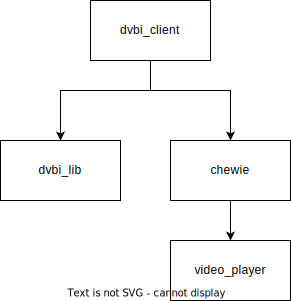
\includegraphics[width=\linewidth]{figures/dvbi_dir_structure}}
	\caption{DVB-I Dependency Structure}
	\label{fig:dvbi_dir_structure}
\end{figure}



This development project utilizes a direct dependency approach to include dependencies into the repository, which allows for quicker changes and bug fixes. The Chewie library is used as a wrapper for the Java Exoplayer and includes two main components: the ChewieController and the MaterialControls UI component. In this project, the Android MaterialControl object is copied and modified to fit the project's specific needs. The customized MaterialControls UI component is initialized as a custom video overlay UI object called MyMaterialControls. Seen in figure \ref{fig:mymaterialcontrols}


\begin{figure}[ht]
	\centerline{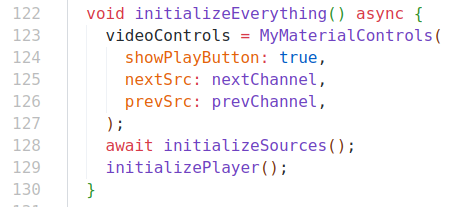
\includegraphics[width=\linewidth]{figures/MyMaterialControls}}
	\caption{Custom video overlay initialization}
	\label{fig:mymaterialcontrols}
\end{figure}


\section{Features DVB-I Parser}


\begin{itemize}
	\item XML to Dart object mapping
	\item Dart objects to JSON (and xml to json)
	\item Command line utility (examples and how it works)
	\item Async http request for parallel fetching
	\item Lazy loading. Only request data you need. Request more on obj access
\end{itemize}


An important part of our implementation is the dvbi parsing library. We created the library to make \emph{http calls}\footnote{\url{https://pub.dev/packages/http}} to the serviceList servers and parse the responses. The responses of the server are in xml format so we used the \emph{xml dart package}\footnote{\url{https://pub.dev/packages/xml}} to parse it into dart and json object for further use. The services of the serviceList i.e.  were parsed into serviceElement objects which contained meta data like servicename, id etc (shown in figure \ref{fig:serviceElmentJSON}). Furthermore they contained schedule and programinfo endpoints which where used to retireve even more meta data. This includes scheduling information and extended program information. The dvb-i parser library is an external dart library and can be seamlessly imported into other projects. Furthermore it uses lazy loading this means that only the requested data you need will be loaded which improves the performance. Dart employs the concept of Asynchronous programming, which includes futures, async, and await. By using asynchronous operations, our program can continue executing tasks while waiting for other long-running operations, such as fetching data over a network, to complete.








%write more about libraries used XML to Dart object mapping
%Features: Lazy loading. Only request data you need. Request more on obj access Async http request for parallel fetchingXML to JSON parsing  


\begin{figure}[ht]
	\centerline{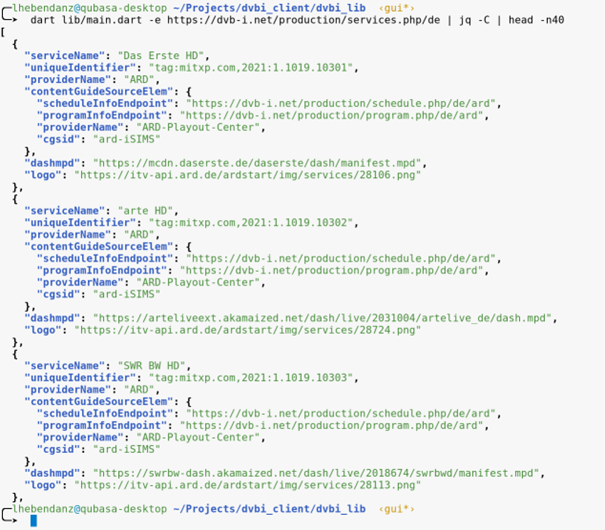
\includegraphics[width=\linewidth, , height=10cm]{figures/serviceElementJSON}}
	\caption{Overview serviceElement json}
	\label{fig:serviceElmentJSON}
\end{figure}




\subsection{DVB-I Parser: Schedule Info}
%schedule info picture oder fett geschrieben

We used the ScheduleInfoEndpoint descirebed in [Quelle: dvbi standard] and shown in figure \ref{fig:scheduleInfoEndpoint} to retrieve scheduleinfo meta data for specific programs .

Every ServiceElement Object of our implementation can request more metadata by accessing the scheduleInfo dart object.
By default the schedule information for the next 6 hours gets fetched on object access.  However, it's easy to extend this time window. To simplify further usage, we parse the duration information of a program from a string to a double. This is necessary because the original string representation follows the ISO 8601-1 format [Quelle], which is not very human-readable.

During implementation, we discovered that the provided endpoint did not return the correct metadata. After conducting several tests with different variations of the endpoint, we found that substituting the word "production" in the URL with "staging" resulted in the correct scheduling information.



%maybe describe mandatory parameters in text or in caption
\begin{figure}[ht]
	\centerline{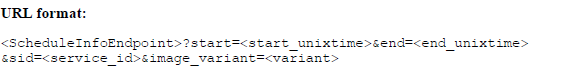
\includegraphics[width=\linewidth]{figures/scheduleInfoEndpointTime}}
	\caption{Overview scheduleInfoEndpoint Quelle:Dvbi einfügen!!!!}
	\label{fig:scheduleInfoEndpoint}
\end{figure}



\subsubsection{DVB-I Parser: Detailed Program Info }



To obtain additional metadata for a specific program of a particular service, we utilized an HTTP request to the ProgramInfo-Endpoint, as depicted in Figure \ref{fig:programInfoEndpoint}. We used the programId (crid), which was obtained through the schedulingInfo request. Similar to the issues encountered during the schedulingInfo request, we faced data problems while using the URL with "production" in the path, and had to replace it with "staging." However, we still encountered a problem where the Endpoint did not respond with all the metadata that could be displayed by the DVB-I Client. We were only able to retrieve a limited amount of additional information, such as the longer text description of the program.

%Problem: Endpoint doesn’t response with all  the metadata that could be displayed by the DVB-I Cient


%maybe describe mandatory parameters in text or in caption
\begin{figure}[ht]
	\centerline{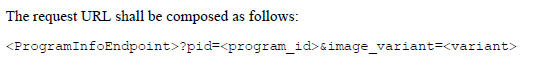
\includegraphics[width=\linewidth]{figures/programInfoEndpoint}}
	\caption{Overview scheduleInfoEndpoint Quelle:Dvbi einfügen!!!!}
	\label{fig:programInfoEndpoint}
\end{figure}


\subsubsection{DVB-I Parser: Optimization}\label{dvbi opt}

Initially, our implementation had a runtime of $O(n^2)$ due to the requirement of matching each ScheduleEvent field with its corresponding program field marked by CRID. This was causing high execution time, as we were iterating through the entire XML tree using the xml dart library.

However, we were able to significantly improve the performance of our program by utilizing a HashMap. This allowed us to retrieve the metadata of each service element at once, reducing the time from 10 minutes to just 30 seconds. It is important to note that this does not mean the user of our application will have to wait for 30 seconds to see any program results, as we use asynchronous functions.







\subsubsection{Gui Application}\label{gui}

libraries used(?)
layout of GUI/Screenshots
Content Guide Page
features: breaks everything 
Channel Browsing
features: subtitles, volume control, next/prev channel, show channel logo and name

\section{Challenges}


 

During the implementation of the DVB-I Parser Library and DVB-I GUI, several challenges were encountered. One significant challenge of the DVB-I parser library, as outlined in Section \ref{dvbi opt}, was the limited scalability when retrieving multiple meta-information for various services and their associated programs. We addressed this challenge by utilizing a hash map and reducing the time interval for displaying programs from the next 24 hours to 6 hours. To prevent long waiting times for users of the DVB-I client, we used the concept of dart streams and asynchronous functions to decrease the loading time for channels.
Another issue faced during the implementation of the DVB-I parser library was the incorrect information response from the official endpoints, as discussed in Section \ref{dvbi_parser}. It appears that the production environment of the endpoint is not up-to-date and needs to be updated soon. 


Furthermore, the responses from the endpoint varied significantly regarding the presence or absence of specific information. This is because the DVB-I standard allows for a wide range of possibilities.
Consequently, our code required robustness and flexibility to handle null values and avoid errors in the client interface.



%still missing, maybe move to gui challenges
State Management in Flutter: 
Unaccounted for Dart language features in Riverpod
Riverpod: Providers + Dart streams = StreamProviders
out-of-the-box state management using State widgets
start and end time

Bugs in libraries: videoplayer, chewie


%Dart Streams, Dart async 
%idea: reduce loading times by asynchr loading channels. 
%DVB-I Server wrong response data with official endpoints ( use of different staging Endpoints for correct data)
%o(n2) performance issue due to the structure of the given xml tree and our used xml lib
%start and end time 
%flexibility in standard leads to many edge cases 

\section{Features GUI}\label{dvbi_parser}


Main branch features:
\begin{itemize}
	\item layout of GUI/Screenshots
	\item mute video stream
	\item next/prev channel
	\item show channel logo and name
\end{itemize}

Content-Guide page branch: 
\begin{itemize}
	\item List of all TV channels with their corresponding logo
	\item Shows what TV show is currently running and a short description
	\item Can be selected to directly jump to the video stream
	\item dynamic loading. Loads the content dynamically into the ui on page scroll 
\end{itemize}



\section{Challenges GUI}

State Management in Flutter is quite convoluted. 

\begin{itemize}
	\item Dart Streams, Dart async
	\item idea: reduce loading times by asynchr loading channels. 
	\item State Management in Flutter: 
	\item Unaccounted for Dart language features in Riverpod
	\item Riverpod: Providers + Dart streams = StreamProviders
	\item out-of-the-box state management using State widgets
\end{itemize}	

\section{Evaluation}


%anforderungen erfüllt? verschiedene programme abspielen auf android tv , anzeigen meta information etc....

%ist our code flexible to various different xml formats for same request? -> yes tested with all service available in the servicelist

\begin{itemize}
	\item scalability
	\item include screenshots cross platform framework flutter ....does it work on android and apples ios?
	\item only android in combination with exoplayer as mpeg dash is not supported by hls and the current flutter videoplayer libs
\end{itemize}



\section{Conclusion and Future Work}

subtitles, channel info button, streaming hls (compatibility with apples ios, not only android), user input start and end time for specific program information



\begin{thebibliography}{00}
\bibitem{b1.1} Flutter, ``Flutter architectural overview``, [Online] \url{https://docs.flutter.dev/resources/architectural-overview}
	
%=============================0%
\bibitem{b1} G. Eason, B. Noble, and I. N. Sneddon, ``On certain integrals of Lipschitz-Hankel type involving products of Bessel functions,'' Phil. Trans. Roy. Soc. London, vol. A247, pp. 529--551, April 1955.
\bibitem{b2} J. Clerk Maxwell, A Treatise on Electricity and Magnetism, 3rd ed., vol. 2. Oxford: Clarendon, 1892, pp.68--73.
\bibitem{b3} I. S. Jacobs and C. P. Bean, ``Fine particles, thin films and exchange anisotropy,'' in Magnetism, vol. III, G. T. Rado and H. Suhl, Eds. New York: Academic, 1963, pp. 271--350.
\bibitem{b4} K. Elissa, ``Title of paper if known,'' unpublished.
\bibitem{b5} R. Nicole, ``Title of paper with only first word capitalized,'' J. Name Stand. Abbrev., in press.
\bibitem{b6} Y. Yorozu, M. Hirano, K. Oka, and Y. Tagawa, ``Electron spectroscopy studies on magneto-optical media and plastic substrate interface,'' IEEE Transl. J. Magn. Japan, vol. 2, pp. 740--741, August 1987 [Digests 9th Annual Conf. Magnetics Japan, p. 301, 1982].
\bibitem{b7} M. Young, The Technical Writer's Handbook. Mill Valley, CA: University Science, 1989.

%change bib structure
@misc{iso2019date,
  title={Date and time—Representations for information interchange—Part 1: Basic rules},
  author={ISO 8601-1: 2019},
  year={2019},
  publisher={ISO—Int Organ Stand}
}



\bibitem{b1.2} Skia 2D, ``Skia 2D Rendering Library``, [Online]
\url{https://skia.org/}

\bibitem{chewie_library} Chewie Library, [Online] 
\url{https://pub.dev/packages/chewie}

\bibitem{video_player_library} Video Player Library, [Online] 
\url{https://pub.dev/packages/video_player}


\bibitem{DVB} Digital Video Broadcasting Project, [Online]
\url{https://dvb.org/}

\bibitem{DVBI-I} Digital Video Broadcasting-Internet: ``a standards-based solution for delivering television – live, linear and on-demand – in the internet age``
\url{https://dvb-i.tv/}

\end{thebibliography}
%\vspace{12pt}
%\color{red}
%IEEE conference templates contain guidance text for composing and formatting conference papers. Please ensure that all template text is removed from your conference paper prior to submission to the conference. Failure to remove the template text from your paper may result in your paper not being published.


\end{document}
